% !TeX spellcheck = de_DE
\chapter{Friedmann-Gleichung\label{chapter:friedmann}}
\lhead{Friedmann-Gleichung}
\begin{refsection}
\chapterauthor{Andri Hartmann und Tobias Schuler}
\lhead{Friedmann-Gleichung}
\rhead{}
\begin{quote}\it
Wir dürfen das Weltall nicht einengen, um es den Grenzen unseres
Vorstellungsvermögens anzupassen, wie der Mensch es bisher zu tun pflegte.
Wir müssen vielmehr unser Wissen ausdehnen, sodass es das Bild des Weltalls
zu fassen vermag.
\end{quote}
\begin{flushright}
--- Sir Francis von Verulam Bacon, 1561 -- 1626
\end{flushright}

In diesem Kapitel möchten wir dem Leser helfen,
{\em das Bild des Weltalls fassen zu vermögen}, wie Francis Bacon sagt.
Um dies zu tun, werden wir versuchen, das Gebilde, welches wir Universum nennen, unter Zuhilfenahme der physikalischen Gesetze in einen mathematischen Kontext zu bringen.

\section{Vorgeschichte}
\rhead{Vorgeschichte}
Mit der Formulierung der Allgemeinen Relativitätstheorie durch Albert Einstein war es erstmals möglich,
sich seriös Gedanken über die Geschichte des
Universums zu machen. An dieses Problem haben sich anfangs der zwanziger Jahre bekannte Wissenschaftler wie Einstein, deSitter, Friedmann und Lemaitre gemacht. 
Zu dieser Zeit gab es wenig bis keine experimentellen Daten, die Aussagen über Geometrie oder Dynamik des Weltalls hätten machen können. So kam es, das unter den führenden Astronomen das Bild eines statischen Universums allgemein üblich war.

Durch die Entdeckung der Fluchtbewegungen von Galaxien mithilfe der Rotverschiebungen gelang es 1929 dem US-amerikanischen Astronomen Edwin Hubble, die damalige Vorstellung eines statischen Kosmos zu widerlegen. Diese Entdeckung hatte zur Folge, dass die Idee eines statischen Universums verworfen wurde. Es stellt sich nun die spannende Frage: Wie ändert sich das Universum mit der Zeit? Und eben diese Frage wird mit der Friedmann-Gleichung beantwortet.
\pagebreak

\section{Voraussetzungen an das Universum}
\rhead{Voraussetzungen}
Damit wir die Friedmann-Gleichung auf das Universum anwenden können, muss das kosmologische Prinzip erfüllt sein. 
\begin{satz}[Kosmologisches Prinzip]
	\label{Prinzip:kosmologisches Prinzip}
	Das kosmologische Prinzip besagt, dass auf einer grossen Längenskala kein Ort im Universum gegenüber einem anderen ausgezeichnet ist. Diese Annahme bedingt zwei Eigenschaften, Isotropie und Homogenität. Isotropie  bezeichnet die Unabhängigkeit einer Eigenschaft von der Richtung, Homogenität die Gleichheit einer physikalischen Eigenschaft über die gesamte Ausdehnung eines Systems.
\end{satz}

\subsubsection*{Was bedeutet nun grosse Längenskala?}
Betrachten wir von der Erde aus den Sternenhimmel, ist das kosmologische Prinzip nicht erfüllt. Wir sehen nämlich ein Sternenbild, was mitnichten auf eine regelmässige Verteilung der Materie hindeutet. Wir sprechen hier von einer Längenskala von hundert bis tausend Parsec\footnote{Ein Parsec ist ein astronomisches Längenmass. Es entspricht etwa 3.26 Lichtjahren.}. Erhöhen wir die Längenskala auf einige hunderttausend Parsec, sodass wir die Milchstrasse und andere Galaxien sehen, ist der Unterschied zwischen Sternen und sternenlosen Gebieten immernoch auszumachen. Erst wenn die Skala eine unvorstellbare Grösse von Millionen bis Milliarden Parsec angenommen hat, ist das kosmologische Prinzip erfüllt. 

\section{Skalenfaktor $a$\label{Section:Skalenfaktor}}
\rhead{Skalenfaktor}
Um ein dynamisches Universum beschreiben zu können, führen wir ein dreidimensionales Koordinatensystem ein, welches sich mit der relativen Bewegung von Galaxien mitbewegen kann. In einem solchen System besitzen die Objekte fixe Koordinaten und sind somit wie in einem Raster eingefroren. Die Einheit des Rasters wird durch den {\em Skalenfaktor} $a$ ausgedrückt und ist eine Funktion der Zeit. In Abbildung \ref{friedmann:friedmannRaster} ist ein solches Raster zum Zeitpunkt $t_0$ und $t_1$ aufgezeichnet. Die Punkte auf dem Raster stellen Galaxien dar. Die Linie zwischen der roten und blauen Galaxie zeigt den Abstand. Dehnt sich das Universum nun aus, dehnt sich das Raster mit. Dies ist in der Abbildung rechts deutlich zu sehen ist. Die Grösse der Galaxien und die Position auf dem Raster bleiben gleich, der Abstand zwischen den Galaxien hat sich aber verändert. 

\begin{figure}
	\centering
	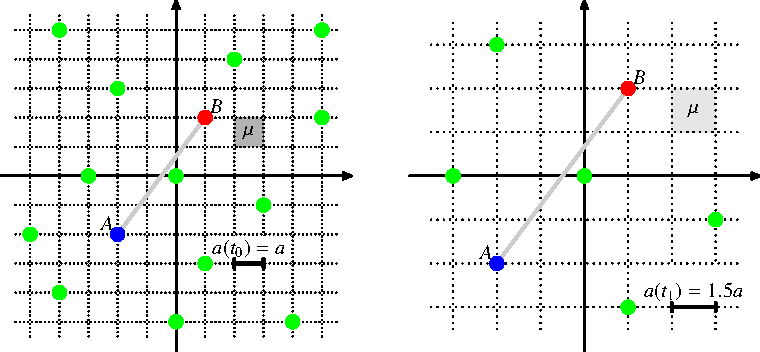
\includegraphics{friedmann/images/friedmann-1.pdf}
	\caption{Raster ums Universum für zwei verschiedene Skalenfaktoren}
	\label{friedmann:friedmannRaster}
\end{figure}%
\subsection{Mathematische Beziehungen im Koordinatensystem \label{friedmann:Beziehungen im Koordinatensystem}}
Die Distanz zwischen zwei Punkten $A$ und $B$ entspricht 
\begin{equation}
D(t)\, = \sqrt{a^2(t)\,\Delta\,x^2 + a^2(t)\,\Delta\,y^2 + a^2(t)\,\Delta\,z^2}\, =\, a(t) \sqrt{\Delta\,x^2 + \Delta\,y^2 + \Delta\,z^2}.
\label{friedmann:Abstand}
\end{equation}
F\"{u}r die Geschwindigkeit, mit der sich die beiden Punkte relativ zueinander bewegen, gilt 
\begin{equation}
v(t) = \dfrac{dD}{dt} 
= \dot{a}(t) \sqrt{\Delta\,x^2 + \Delta\,y^2 + \Delta\,z^2}.
\label{friedmann:geschwindigkeit}
\end{equation}
Um nun Aussagen über die Dynamik des Universums zu machen, die nicht von der willkürlichen Wahl des Skalenfaktors abhängen, teilen wir die Geschwindigkeit $v(t)$ durch die Distanz $D(t)$. Schlussendlich ist das Ziel, eine Seite der hergeleiteten Gleichung in diese Form zu bringen:
\begin{equation}
\frac{v}{D} = \frac{\dot{a}}{a}.
\end{equation}
Gemäss Satz \ref{Prinzip:kosmologisches Prinzip} und der Eigenschaft unseres Koordinatensystems, beschrieben in Abschnitt \ref{Section:Skalenfaktor}, bleibt die Masse in einem Einheitswürfel konstant über die Zeit. Somit ist die Masse $M$ in einem Würfel mit Dimension $\Delta x$, $\Delta y$ und $\Delta z$ 
\begin{equation}
M_{xyz} = \mu \,\Delta x \,\Delta y \,\Delta z.
\end{equation}
Der Parameter $\mu$ sagt aus, wieviel Masse in einem Einheitswürfel vorhanden ist. Er ist von der Wahl der Rastergrösse zum Zeitpunkt $t_0$ abhängig, jedoch konstant über die Zeit. Das Volumen des Würfels ist bekanntlich
\begin{equation}
V_{xyz} = a^3 \,\Delta x \,\Delta y \,\Delta z
\end{equation}
und folglich kann die Massendichte geschrieben werden als
\begin{equation}
\rho = \frac{M_{xyz}}{V_{xyz}} = \frac{\mu}{a^3}.
\label{friedmann:dichte}
\end{equation}
Zu beachten ist, dass die Dichte abhängig von der Ausdehnung des Skalenfaktors ist. Der Einheitswürfel in Abbildung \ref{friedmann:friedmannRaster} zum Zeitpunkt $t_1$ ist im Vergleich zum Zeitpunkt $t_0$ grösser geworden, weil sich das Raster ausgedehnt hat. Die Masse im Würfel hat aber nicht zugenommen und bleibt $\mu$. Das bedeutet, dass die Dichte abgenommen haben muss. Rechts ist diese Abnahme mit dem helleren Grau verdeutlicht. Die Ausdehnung geschieht in einem dreidimensionalen System kubisch, die Massendichte $\rho$ nimmt also kubisch ab.

\section{Alexander Friedmann und Georges Lema\^{i}tre}
\rhead{Friedmann und Lema\^{i}tre}
Die Friedmann-Gleichung beschreibt das Verhalten des Universums nach der Inflation des Kosmos im Rahmen des Standard-Urknall-Modells. Da Alexander Friedmann und Georges Lema\^{i}tre die Gleichung unabhängig voneinander entdeckten, wird sie manchmal auch als Friedmann-Lema\^{i}tre-Gleichung bezeichnet. Die {\em Energiedichte} $\rho$, die {\em Krümmung} $\kappa$ und die {\em kosmologische Konstante} $\Lambda$ sind die Parameter der Gleichung
\begin{equation}
\left(\frac{\dot{a}}{a}\right) ^2 = \frac{8 \pi G}{3} \rho - \frac{\kappa c^2}{a^2} + \frac{\Lambda c^2}{3}.
\end{equation}
Bevor wir beginnen, die Gleichung herzuleiten (siehe Abschnitt \ref{friedmann:subsec:Herleitung der Gleichung}), können wir schon jetzt verschiedene Lösungen für unterschiedliche Parameterwerte diskutieren. Das hilft uns später beim Rekonstruieren der Geschichte des Universums.

\subsection{Masseloses Universum \label{friedmann:masselosesUniversum}}
Setzen wir $\rho = 0$, entspricht dies einem masselosen Universum.  Wir schreiben die Gleichung ohne den ersten Term
\[\left(\frac{\dot{a}}{a}\right) ^2 = - \frac{\kappa c^2}{a^2} + \frac{\Lambda c^2}{3}\]
Für beide Terme auf der rechten Seite lässt sich die Differentialgleichung in geschlossener Form lösen, man kann so ein ungefähres Bild vom Verhalten der allgemeinen Lösung erhalten.
\begin{enumerate}
	\item $\kappa = 0$ :
		\begin{align}
			\nonumber \left(\frac{\dot{a}}{a}\right) ^2 &= \frac{\Lambda c^2}{3} \\
			\nonumber \dot{a} ^2 &= \frac{\Lambda c^2 a^2}{3}  \\
			\nonumber \dot{a} &= \underbrace{\sqrt{\frac{\Lambda c^2}{3}}}_{\displaystyle=E} a \\
			\nonumber \dot{a} &= E \cdot a \\
			a &= a_0 \cdot e^{E \: t} \label{friedmann:Lambda}
		\end{align}
	
	
Mit $\kappa = 0$ gibt es zwei mögliche Ausprägungen für das Universum, entweder ist $E = 0$ oder $E > 0$. Im ersten Fall wäre das Universum statisch und für alle Zeit gerade so gross wie $a_0$. Im zweiten Fall würde sich das Universum exponentiell ausdehnen.
		
	\item $\Lambda = 0$ :
		\begin{align}
			\nonumber \left(\frac{\dot{a}}{a}\right) ^2 &= - \frac{\kappa c^2}{a^2}\\
			\nonumber \dot{a} ^2 &= - \kappa \, c^2 \\
			\nonumber \dot{a} &= \sqrt{- \kappa}\, c \\
			a &= \sqrt{- \kappa}\, c \cdot t + a_0\label{friedmann:Kappa}
		\end{align}
		
Auch hier gibt es zwei mögliche Ausprägungen. Wenn $\kappa = 0$, dann ist das Universum statisch und hat für alle Zeit den Skalenfaktor $a_{0}$, wenn $\kappa > 0$ wächst der Skalenfaktor linear mit der Zeit.
	
\end{enumerate}

\subsection{Universum mit Masse \label{friedmann:UniversumMitMasse}} 
Wie vorher schon angedeutet, steht $\rho$ für die Dichte des Universums. Ist das Universum masselos, ist die Dichte 0. Gehen wir aber davon aus, dass im Universum Materie vorhanden ist, findet man eine weitere Lösung der Differentialgleichung. Damit die Gleichung lösbar ist, vernachlässigen wir den $\Lambda$- und $\kappa$-Term. Für die Dichte setzen wir (\ref{friedmann:dichte}) ein:
\begin{align}
	\nonumber\left(\frac{\dot{a}}{a}\right) ^2 &= \frac{8 \pi G}{3} \frac{\mu}{a^3}. \\
	\intertext{Weiter können wir $\mu$ so wählen, dass sich der konstante Term als eins schreiben lässt:}
	\nonumber \left(\frac{\dot{a}}{a}\right) ^2 &= \frac{1}{a^3}. \\
	\intertext{Um die Gleichung zu lösen, ziehen wir die Quadratwurzel und multiplizieren mit $a$:}
	\nonumber \dot{a} = \frac{da}{dt} &=\frac{1}{\sqrt{a}}. \\
	\intertext{Ab dem nächsten Schritt betrachten wir $t$ als von $a$ abhängige Variable:}
	\nonumber \frac{dt}{da} &= \sqrt{a} \\
	\nonumber t &= \frac{2}{3} a^{3/2} \\
	a &= \frac{3}{2} t^{2/3}. \label{friedmann:Masse}
\end{align}

\subsubsection{Diskussion der Lösungen}
Wir finden also für jeden Term in der Gleichung eine andere Beschreibung der Bewegung des Universums. Betrachten wir die Anfangsgleichung genauer, können wir herauslesen, welcher Term bei einer gegebenen Grösse $a$ dominiert.
\begin{alignat}{5}
	\left(\frac{\dot{a}}{a}\right) ^2 &= \;\; &\frac{8 \pi G}{3}&\;\rho\; &-\;\frac{\kappa c^2}{a^2}\; &+ \;\frac{\Lambda c^2}{3}\\
	\intertext{Wir setzen für $\rho$ den Ausdruck aus (\ref{friedmann:dichte}) ein:}
	\left(\frac{\dot{a}}{a}\right) ^2 &= \;\;&\frac{8 \pi G}{3} &\frac{\mu}{a^3}\; &-\;\frac{\kappa c^2}{a^2}\; &+\; \frac{\Lambda c^2}{3}.
\end{alignat}
Für kleine Werte von $a$ wird der $\rho$-Term dominieren, für mittlere Werte von $a$ der $\kappa$-Term, und für grosse Werte dominiert der $\Lambda$-Term. Das heisst, die Lösungen setzen sich in zeitlicher Reihenfolge wie folgt zusammen: (\ref{friedmann:Masse})  dominiert zu Beginn, dann mischt sich (\ref{friedmann:Kappa}) ins Spiel, und am Schluss dominiert (\ref{friedmann:Lambda}) über das Schicksal des Universums. In Abbildung \ref{friedmann:mathematischFriedmann} ist die numerische Lösung der Differentialgleichung mit allen Termen eingezeichnet.
Zu bemerken ist, dass die Abbildung rein qualitativ veranschaulicht ist, da wir die Parameterwerte zur einfacheren Betrachtung angepasst haben. Ohnehin führen diese Anpassungen aber nicht zu einer falschen Vorstellung der Bedeutsamkeit der Terme, da diese nur die Vorfaktoren, nicht aber die Potenzen beeinflussen. 
\begin{figure}[h]
	\centering
	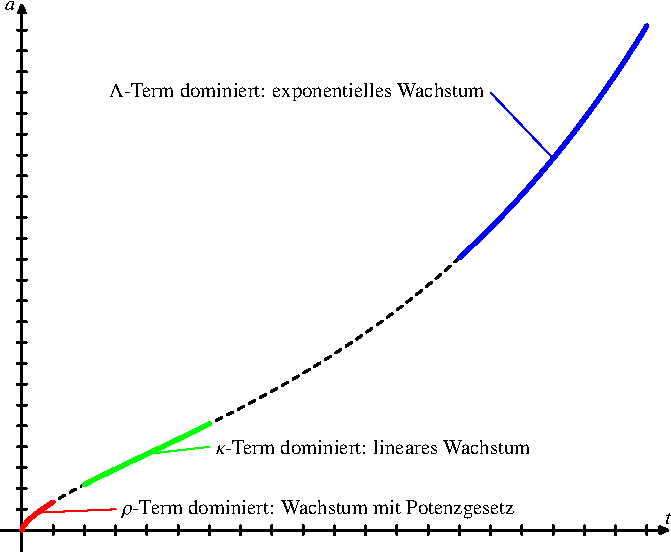
\includegraphics{friedmann/images/friedmann-2.pdf}
	\caption{Mathematische Bedeutung für die Ausbreitung des Universums der einzelnen Terme}
	\label{friedmann:mathematischFriedmann}
\end{figure}%
\subsection{Herleitung der Differentialgleichung \label{friedmann:subsec:Herleitung der Gleichung}}
Im folgenden Abschnitt versuchen wir die Bedeutung der einzelnen Terme physikalisch zu hinterlegen. Das ist nicht immer einfach, denn die Differentialgleichung befasst sich unter anderem mit den Einsteinschen Feldgleichungen. Trotzdem werden wir in diesem Kapitel einige interessante Relationen mithilfe der klassischen Physik herleiten.
\subsubsection{Newtonscher Ansatz}
Um die relative Beschleunigung zweier Punkte im Universum zu beschreiben, wird von folgendem Ansatz ausgegangen: Ein Beobachter befindet sich im Ursprung des Koordinatensystems und ist in Ruhe. Um nun die Kraft auf einen Körper der {\em Masse} $m$ im {\em Abstand} $D$ zu berechnen, denkt man sich eine Kugelschale um den Ursprung mit {\em Radius} $D$. Die Kraft auf den Körper verhält sich wie die Punktmasse aller  einzelnen Körper in der Kugel im Ursprung gedacht. Abbildung \ref{friedmann:gravitation}s illustriert genau dieses Szenario.
\begin{figure}[h]
	\centering
	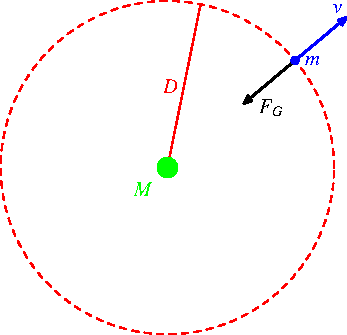
\includegraphics{friedmann/images/friedmann-5.pdf}
	\caption{Modell für den Newtonschen Ansatz
	\label{friedmann:gravitation}}
\end{figure}%
Im Folgenden werden die in  Abschnitt \ref{friedmann:Beziehungen im Koordinatensystem} hergeleiteten Formeln angewendet. Einfachheitshalber schreiben wir für den Abstand im Raster
\[
R
:=
\sqrt{\Delta x^2 + \Delta y^2 + \Delta z^2}
\]
und für das Volumen V der Kugel
\[V_\text{Kugel} = \frac{4 \pi }{3} a^3 R^3.\]
Gemäss Newton ergibt sich die Gravitationskraft aus
\begin{equation}
F_G = -\frac{m M G}{D^2}.
\end{equation}
Da die Gravitationskraft zwecks Vereinfachung des Modells als einzige Kraft wirkt, gilt für die Beschleunigung $A$ (Hier $A$, weil der Kleinbuchstabe $a$ für den Skalenfaktor reserviert ist.) von $m$ mit $F = m A$ :
\[A = - \frac{M G}{D^2} = \ddot{a} R \quad\Leftrightarrow\quad \ddot{a} = -\frac{M G}{a^2 R^3} \quad\Leftrightarrow\quad \frac{\ddot{a}}{a} = -\frac{\frac{4 \pi }{3} M G}{\frac{4 \pi}{3}a^3 R^3} \quad\Leftrightarrow\quad \frac{\ddot{a}}{a} = -\frac{4 \pi G}{3} \frac{M}{V_\text{Kugel}}.\]
Die Gleichung wurde so angepasst, dass im Zähler die Masse und im Nenner das Volumen steht, was der Dichte entspricht. Damit vereinfacht sich die Beschleunigung zu
\begin{equation}
\frac{\ddot{a}}{a} = -\frac{ 4 \pi G}{3} \rho.
\end{equation}
\subsubsection{Bedeutung der Beschleunigungsgleichung}
Setzt man für die Dichte den Ausdruck aus (\ref{friedmann:dichte}) ein ergibt sich
\[\frac{\ddot{a}}{a} = -\frac{ 4 \pi G}{3} \frac{\mu}{a^3}.\]
Durch geschickte Wahl der Masseinheiten kann $\mu$ den konstanten Faktor auf der rechten Seite durch eins ersetzen. So vereinfacht sich die Gleichung zu
\[\frac{\ddot{a}}{a} = -\frac{1}{a^3} \qquad\Leftrightarrow\qquad \ddot{a} = -\frac{1}{a^2}.\]
Die Differentialgleichung ist nichtlinear und nicht in geschlossener Form lösbar. Trotzdem können wir gewisse Aussagen machen, nämlich
\begin{enumerate}
	\item Die negative Beschleunigung wirkt der Ausdehnung des Universums entgegen. 
	\item Ein statisches Universum ist nicht möglich für $\rho \neq 0$.
	\item Die Formel hängt nicht vom Ort $R$ ab, was bedeutet, dass unser Ansatz mit dem Beobachter im Ursprung legitim war.
\end{enumerate}

\subsubsection{Energieerhaltung}
Da wir versuchen, das Universum als ein geschlossenes physikalisches System zu beschreiben, muss auch hier der wichtige Satz der Energieerhaltung gelten. Wir befassen uns wieder mit dem Modell in Abbildung \ref{friedmann:gravitation}. Die Masse $m$ ist nicht im Ruhestand, sondern entfernt sich mit der Geschwindigkeit $v$ von der Masse $M$. Betrachten wir für den Anfang die Beziehung zwischen kinetischer und potentieller Energie:
\begin{equation}
E_{\text{ges}} = E_{\text{kin}} - E_{\text{pot}} =  \frac{m v^2}{2} - \frac{m M G }{D}.
\end{equation}
Wir werden später noch andere Formen von Energie kennenlernen, die wir dieser Gleichung hinzufügen müssen. Doch beginnen wir in kleinen Schritten. Die Gesamtenergie kann nun drei wesentliche, für die Dynamik interessante Werte annehmen, nämlich
\begin{enumerate}
	\item $E_{\text{ges}} > 0 \rightarrow$ Eine Masse $m$ entflieht der Schwerkraft.
	\item $E_{\text{ges}} = 0 \rightarrow$ Eine Masse $m$ nähert sich asymptotisch  der Geschwindigkeit null, bleibt aber nie stehen. (Fluchtgeschwindigkeit)
	\item $E_{\text{ges}} < 0 \rightarrow$ Eine Masse $m$ wird so stark angezogen, dass die Geschwindigkeit ihre Richtung ändert.
\end{enumerate}
Nennen wir die Gesamtenergie $E_{\text{ges}}$ eine Konstante $E$ und formen die Gleichung um:

\begin{align*}
	\frac{m v^2}{2} - \frac{m M G}{D} &= E_1 \\ 
	v^2 - \frac{2 M G}{D} &= \underbrace{\frac{2E_1}{m}.}_{\displaystyle E_2} \\	
	\intertext{Wir setzen (\ref{friedmann:geschwindigkeit}) und (\ref{friedmann:Abstand}) ein:}
	\left( \dot{a} \, R\right)^2 &= \frac{2 M G}{a\,R} + E_2 \\
	\frac{\dot{a}^2}{a^2} &= \frac{2 M G}{a^3 R^3} + \frac{E_2}{a^2 R^2} \\
	\left(\frac{\dot{a}}{a} \right)^2 &= \frac{\displaystyle\frac{4 \pi}{3}2 M G}\displaystyle{\frac{4 \pi}{3} a^3 R^3} + \frac{E_2}{a^2 R^2}.
\end{align*}
Auf der rechten Seite der Gleichung erscheint jetzt die Masse der Kugel mit Radius $R$ dividiert durch das Kugelvolumen $V$, was der Dichte entspricht. Daraus resultiert die vereinfachte Differentialgleichung 
\begin{equation}
\left(\frac{\dot{a}}{a} \right)^2 = \frac{8 \pi G}{3} \rho + \frac{E_2}{a^2 R^2}.
\label{friedmann:EnergieerhaltungUniversum}
\end{equation}
Für die Dichte $\rho$ setzen wir den Ausdruck aus (\ref{friedmann:dichte}) ein:
\[\left(\frac{\dot{a}}{a} \right)^2 = \frac{8 \pi G}{3} \frac{\mu}{a^3} + \frac{E_2}{a^2 R^2}. \\\]
Wir wählen die Konstanten $\mu$ und $R$ so, dass die Gleichung folgendermassen vereinfacht wird:
\begin{equation}
\left(\frac{\dot{a}}{a} \right)^2 = \frac{1}{a^3} + \frac{E}{a^2}.
\end{equation}

\subsection{Diskussion der Differentialgleichung}
Wir erinnern uns, die Konstante $E$ steht für die Gesamtenergie des Universums und kann positiv, negativ oder null sein.
\begin{enumerate}
	\item Beginnen wir mit dem einfachsten Fall und setzen $E = 0$.
	\[\left(\frac{\dot{a}}{a} \right)^2 = \frac{1}{a^3}\]
	Diese Gleichung wurde in \ref{friedmann:UniversumMitMasse} schon gelöst. Ist die Gesamtenergie $E$ null, dehnt sich das Universum gemäss  (\ref{friedmann:Masse}) aus. Je grösser also das Universum wird, desto kleiner wird die Geschwindigkeit der Ausdehnung.
	\[\lim_{t\to\infty} \dot{a}(t) = 0\]
	\item Für den zweiten Fall ist $E > 0$.
	\[\ \left(\frac{\dot{a}}{a} \right)^2 = \frac{1}{a^3} + \frac{E}{a^2}\]
	Betrachten wir die rechte Seite, bemerken wir den Potenzunterschied im Nenner. Daraus folgt, dass für {\em kleine} $a$'s der {\em erste} Term dominiert, während der {\em zweite} Term für {\em grosse} $a$'s dominiert. Das kleine Universum verhält sich also wie für $E = 0$. Das grosse Universum hingegen verhält sich wie das massenlose Universum in \ref{friedmann:masselosesUniversum} mit $\Lambda = 0$.  
	
	\item Als letztes soll $E < 0$ sein
	\[\ \left(\frac{\dot{a}}{a} \right)^2 = \frac{1}{a^3} - \frac{|E|}{a^2} \qquad \Leftrightarrow \qquad \dot{a}^2 = \frac{1}{a} - |E|\]
	\begin{equation}
	\dot{a} = \pm \sqrt{\frac{1}{a} - |E|}
	\end{equation}
	Diese Gleichung ist wiederum nicht in geschlossener Form lösbar. Mithilfe des Phasenportraits in Abbildung \ref{friedmann:phasenportrait} kann die Lösung aber ausgearbeitet werden. Wir konzentrieren uns zuerst auf die Kurven und Pfeile für den Energiewert $E = -\frac{1}{2}$. Da die Differentialgleichung nichtlinear ist, entstehen zwei Phasenportraits.  Die rote Kurve beschreibt die Funktion \[f(a) = + \sqrt{\frac{1}{a} - \frac{1}{2}},\] die blaue Kurve $-f(a)$. Die Pfeile im grau hinterlegten Bereich zeigen, wie sich der Skalenfaktor für $f(a)$ und $-f(a)$ verhält. Je länger ein Pfeil ist, desto grösser ist die Veränderung. Die Länge des Pfeils entspricht der Länge der jeweiligen vertikalen roten oder blauen Linie. Gehen wir von der Anfangsbedingung $a_0 = 0^+$ aus, können wir folgende Überlegung machen:
	Das Universum dehnt sich am Anfang ziemlich stark aus, da $a$ klein ist. Irgendwann mischt sich die Gesamtenergie $E$ ins Spiel, die Expansion wird mehr und mehr ausgebremst. Die Geschwindigkeit der Ausdehnung erreicht den Wert null, sobald sich die beiden Terme unter der Wurzel aufheben. Das Universum kommt also zum Stillstand. 
	Die spannende Frage ist, was auf diesen Stillstand folgt. Bleibt das Universum ewig stehen oder dehnt es sich sogar weiter aus? Rein mathematisch gesehen sind beide Fälle durchaus möglich. Wenden wir aber die physikalischen Gesetze an, kommen wir zum Schluss, dass diese Situation nicht stabil sein kann und das Universum gemäss dem blauen Phasenportrait kontrahiert. Dieses Szenario wird Big-Crunch genannt. In grüner Farbe ist genau dieser Big-Crunch dargestellt. 
		
	Die transparenten Linien zeigen den Big-Crunch für unterschiedliche Energiewerte. Dabei gilt: Je grösser die negative Energie ist, desto weniger gross wird das Universum:
	\[\frac{1}{a_\text{Ruhe}} - |E| = 0 \qquad\Leftrightarrow \qquad \frac{1}{a_\text{Ruhe}} = |E| \qquad\Leftrightarrow\qquad a_\text{Ruhe} = \frac{1}{|E|}.\]
\end{enumerate}

\begin{figure}
	\centering
	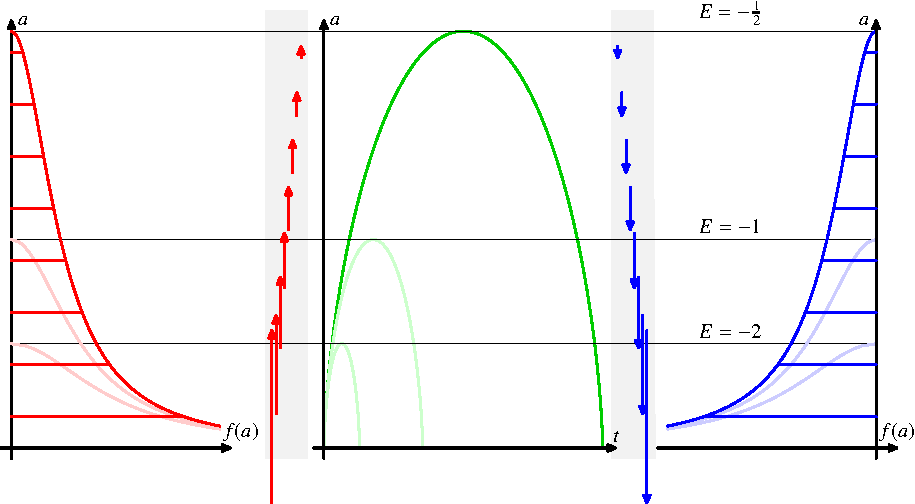
\includegraphics[width  = \textwidth]{friedmann/images/friedmann-6.pdf}
	\caption{Phasenportrait in Abhängigkeit der Gesamtenergie E
		\label{friedmann:phasenportrait}}
\end{figure}%
In der Abbildung \ref{friedmann:universumMasse} sind die drei Szenarien eingezeichnet. Wiederum dient die Grafik der qualitativen Ansicht, die Parameter für $E$ wurden frei gewählt. Die Dominanz der einzelnen Terme ist gemäss den oben beschriebenen Fällen sehr gut auszumachen. Das Universum verhält sich so, wie am Anfang dieses Kapitels beschrieben wurde.

\begin{figure}[h]
	\centering
	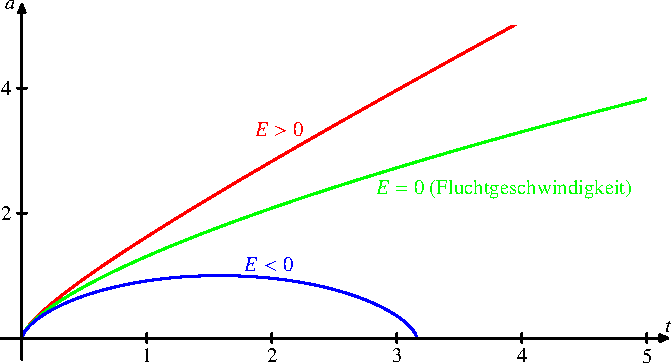
\includegraphics{friedmann/images/friedmann-4.pdf}
	\caption{Verhalten des Universums in Abhängigkeit der Gesamtenergie $E$
		\label{friedmann:universumMasse}}
\end{figure}%

\subsection*{Energiedichte}
Wie wir wissen, existiert im Weltall nicht nur sichtbare, sondern auch dunkle Materie und Strahlung. Dunkle Materie verhält sich in Bezug auf die gravitative Wirkung ähnlich wie sichtbare Materie, und deshalb wird im Folgenden nicht weiter darauf eingegangen.
Anders verhält es sich mit der Strahlung in Bezug auf die Dynamik des Universums. Wir schreiben
\[ E_\text{str} = \frac{h c}{\lambda} \]
wobei $h$ die {\em Planksche Konstante}, $c$ die {\em Lichtgeschwindigkeit} und $\lambda$ die {\em Wellenlänge} des Photons ist.
Nun ist die Energie der Strahlung (z.B. eines Photons) in einem sich ausdehnenden Universum nicht konstant, sondern ändert sich mit der Zeit. 
Denn, vergrössert sich die Raumzeit während der Laufzeit, so geschieht dies auch mit der Wellenlänge des Strahls. Das bedeutet, dass die Energie eines Photons umgekehrt proportional zum Skalenfaktor $a$ ist. Für die Energiedichte der Strahlung bedeutet dies, dass sie sich nicht nur kubisch wie bei der baryonischen Materie ändert, sondern mit vierter Potenz:
\begin{equation}
\rho_\text{str} = \frac{\mu_{\text{str}}}{a^4}.
\end{equation}
In die Energieerhaltung des Universums (\ref{friedmann:EnergieerhaltungUniversum}) setzen wir $\rho_\text{str}$ ein:
\[\left(\frac{\dot{a}}{a} \right)^2 = \frac{8 \pi G}{3} \frac{\mu_{\text{str}}}{a^4} + \frac{E_2}{a^2 R^2}.\]
Wir wählen die Konstanten $\mu_{\text{str}}$ und $R$ so, dass die Gleichung vereinfacht wird zu
\[\left(\frac{\dot{a}}{a} \right)^2 = \frac{1}{a^4} + \frac{E}{a^2} \qquad \Leftrightarrow \qquad\dot{a} = \sqrt{\frac{1}{a^2} + E}.\]
Wiederum ist die Differentialgleichung nicht elementar lösbar. Trotzdem können wir sagen, dass für {\em kleine} $a$'s der erste Term dominiert, während der zweite Term für {\em grosse} $a$'s dominiert. Setzen wir die Gesamtenergie des Universums $E$ gleich null, findet sich die neue Gleichung für den dominierenden ersten Term:
\begin{align}
	\nonumber\left(\frac{\dot{a}}{a} \right)^2 &= \frac{1}{a^4}.\\
	\intertext{Um die Gleichung zu lösen, ziehen wir die Quadratwurzel und multiplizieren mit $a$:}
	\nonumber\dot{a} = \frac{da}{dt} &=\frac{1}{a}.\\
	\intertext{Ab dem nächsten Schritt betrachten wir wieder $t$ als von $a$ abhängige Variable:}
	\nonumber\frac{dt}{da} &= a\\
	\nonumber t &= \frac{1}{2} a^{2}\\
	a &= \sqrt{2}\,t^{1/2}. 
\end{align}
Analog zum Newtonschen Ansatz verhält sich das Universum für einen dominierenden zweiten Term gemäss (\ref{friedmann:Kappa}). 
Im Vergleich mit dem Universum, bei der die gewöhnliche Materie dominiert, ist vor allem zu Beginn ein Unterschied auszumachen. Die Strahlung lässt das Universum am Anfang viel schneller expandieren, siehe Abbildung \ref{friedmann:strahlungMaterie}. 

\begin{figure}
	\centering
	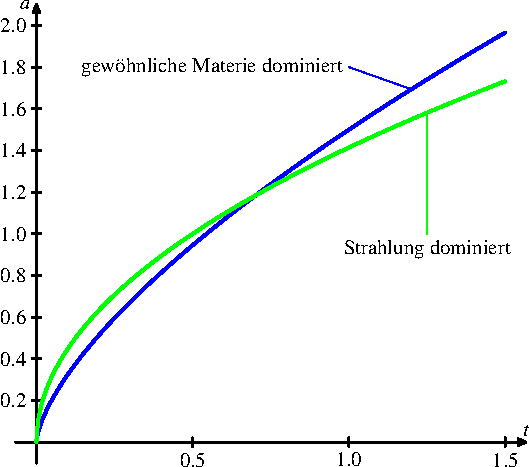
\includegraphics{friedmann/images/friedmann-3.pdf}
	\caption{Strahlung und Materie im Vergleich
		\label{friedmann:strahlungMaterie}}
\end{figure}

\subsection{Geometrie des Raumes}
Die bisher gemachten Überlegungen berücksichtigen nur die klassische oder newtonsche Physik, tatsächlich spielen die relativistischen Gesetze Einsteins eine wesentliche Rolle bei der Beschreibung des Universums. Einsteins Gesetze verknüpfen die Krümmung des Raumes mit dem newtonschen Energieterm. Der Bezeichnung des Energieterms (\ref{friedmann:EnergieerhaltungUniversum}) ändert folgendermassen:  
\begin{equation}
	\left(\frac{\dot{a}}{a}\right) ^2 = \;\frac{8 \pi G}{3} \rho \; -\;\frac{\kappa c^2}{a^2}.
\end{equation}
Der $\kappa$-Parameter beschreibt die Krümmung des Raumes und ist in Tabelle \ref{friedmann:GeometrieDesRaumes} erklärt. Die Krümmung des Raumes kann durch Messen von Winkelsummen im Dreieck bestimmt werden.
\begin{table}[h]
\centering
\begin{tabular}{|>{$}r<{$}|>{$}l<{$}|>{$}c<{$}|}
\hline
\kappa&\text{Geometrie}&\text{Winkelsumme}\: \Delta\\
\hline
+1 & \text{Elliptisch} & > 180^\circ\\
0  & \text{Euklidisch} & =180^\circ\\
-1 & \text{Hyperbolisch} & <180^\circ\\
\hline	
\end{tabular}
\caption{Bedeutung von $\kappa$ für die Geometrie des Raumes\label{friedmann:GeometrieDesRaumes}}
\end{table}
Mathematisch gesehen hat der $\kappa$-Term abgesehen vom Vorzeichen die gleiche Bedeutung wie die Gesamtenergie des Universums, die in \ref{friedmann:EnergieerhaltungUniversum} behandelt wurde, nämlich:
\begin{itemize}
	\item $\kappa = 0$ : Das Universum dehnt sich immer weiter aus. Die Geschwindigkeit der Ausdehnung nähert sich asymptotisch dem Wert null. 
	\item $\kappa = - 1$ : Das Universum verhält sich zuerst, als ob $\kappa$ null wäre. Danach breitet es sich linear aus. Die Geschwindigkeit ist dabei für alle Zeit konstant.
 	\item $\kappa = + 1$ : Das Universum wird grösser und grösser. Die Zunahme nimmt aber immer mehr ab, bis die Geschwindigkeit null wird. Dann fällt es wieder in sich zusammen. Wir sprechen vom Big-Crunch. 
\end{itemize}

Zusammengefasst ist zu sagen, dass ein statisches Universum nur möglich ist, wenn sich keine Materie im Universum befindet und $\kappa = 0$ ist. Da unser Universum nicht leer ist, muss es dynamisch sein. Damit kommen wir zur Frage, was der $\Lambda$-Term bedeutet.

\subsection{Dunkle Energie}
In der Einleitung haben wir geschrieben, dass die Astronomen zuerst von einem statischem Universum ausgingen. Ein statisches Universum ist aber nicht möglich. Um der Dynamik der Gesetze von Newton und Einstein entgegenzuwirken, führte Einstein in seinen Feldgleichungen den $\Lambda$-Term ein, welcher zum $\Lambda$-Term in der Friedmann-Gleichung führt. Einstein bezeichnete diesen Fehler später als die grösste Eselei seines Lebens. In erster Linie wurde der $\Lambda$-Term also gebraucht, um ein statisches Universum zu erzwingen. Heute hat der Term aber eine andere Bedeutung und kann nicht vernachlässigt werden. Man hat den Effekt gemessen, dass das Universum nicht nur linear zunimmt, sondern einen exponentiellen Anstieg verzeichnet. Genau diese exponentielle Lösung resultiert aus dem $\Lambda$-Term. Wir wissen nicht, was es ist, darum nennen wir es dunkle Energie. Wir können aber sagen, dass diese dunkle Energie anti-gravitativ wirken muss.
\end{refsection}
